%------------------------------------------------------------------------------------
\section{Current Flow Preprocessor}

The preprocessor is used for drawing the problems geometry, defining
materials, and defining boundary conditions. The process of construction of current
flow problems is mechanically nearly identical to the construction of
magnetics problems--refer to Sections~\ref{pencil} through~\ref{coffee} for
an overview of the FEMM editing and problem creation commands. This section
considers those parts of problem definition that are unique to current flow problems.

\subsection{Problem Definition}

The definition of problem type is specified by choosing the
\texttt{Problem} selection off of the main menu. Selecting this
option brings up the Problem Definition dialog, shown in
Figure~\ref{cfig5}.

\begin{figure}[htbp]
\centerline{\includegraphics{cd1.ps}}
\caption{Problem Definition dialog.}
\label{cfig5}
\end{figure}

The first selection is the \texttt{Problem Type} drop list. This
drop box allows the user to choose from a 2-D planar problem (the
\texttt{Planar} selection), or an axisymmetric problem (the
\texttt{Axisymmetric} selection).

Next is the \texttt{Length Units} drop list. This box identifies
what unit is associated with the dimensions prescribed in the
model's geometry. Currently, the program supports inches,
millimeters, centimeters, meters, mils, and $\mu $meters.

The first edit box, {\tt Frequency, Hz}, denotes the frequency at 
which the problem is to be analyzed. 

The second edit box is the \texttt{Depth} specification. If a Planar
problem is selected, this edit box becomes enabled. This value is
the length of the geometry in the ``into the page'' direction. This
value is used for scaling integral results in the post processor
(e.g. force, inductance, etc.) to the appropriate length. The units
of the Depth selection are the same as the selected length units.

The second edit box is the \texttt{Solver Precision} edit box. The
number in this edit box specifies the stopping criteria for the
linear solver. The linear algebra problem could be represented by:

\begin{equation}
M x = b
\end{equation}

\noindent
where $M$ is a square matrix, $b$ is a vector, and $x$ is a vector of
unknowns to be determined. The solver precision value determines the maximum
allowable value for $\vert \vert b - Mx\vert \vert / \vert \vert b\vert
\vert $. The default value is $10^{ - 8}$.

The third edit box is labeled {\tt Min Angle}.  The entry in this box is used as a
constraint in the Triangle meshing program.  Triangle adds points to the mesh to
ensure that no angles smaller than the specified angle occur. If the minimum angle
is 20.7 degrees or smaller, the triangulation algorithm is theoretically guaranteed to
terminate (assuming infinite precision arithmetic -- Triangle may
fail to terminate if you run out of precision).  In practice, the
algorithm often succeeds for minimum angles up to 33.8 degrees.
For highly refined meshes, however, it may be necessary to reduce
the minimum angle to well below 20 to avoid problems associated
with insufficient floating-point precision.  The edit box will accept
values between 1 and 33.8 degrees.

Lastly, there is an optional \texttt{Comment} edit box. The user
can enter in a few lines of text that give a brief description of
the problem that is being solved. This is useful if the user is
running several small variations on a given geometry. The comment
can then be used to identify the relevant features for a particular
geometry.

\subsection{Definition of Properties}

To make a solvable problem definition, the user must identify boundary
conditions, block materials properties, and so on. The different types of
properties defined for a given problem are defined via the
\texttt{Properties} selection off of the main menu.

When the \texttt{Properties} selection is chosen, a drop menu
appears that has selections for Materials, Boundary, Point, and
Conductors. When any one of these selections is chosen, the dialog
pictured in Figure~\ref{cfig7} appears.

\begin{figure}[htbp]
\centerline{\includegraphics{hpropdef.ps}}
\caption{Property Definition dialog box.}
\label{cfig7}
\end{figure}

This dialog is the manager for a particular type of properties. All
currently defined properties are displayed in the \texttt{Property
Name} drop list at the top of the dialog. At the beginning of a new
model definition, the box will be blank, since no properties have
yet been defined. Pushing the \texttt{Add Property} button allows
the user to define a new property type. The \texttt{Delete
Property} button removes the definition of the property currently
in view in the \texttt{Property Name} box. The \texttt{Modify
Property} button allows the user to view and edit the property
currently selected in the \texttt{Property Name} box. Specifics for
defining the various property types are addressed in the
following subsections.

\subsubsection{Point Properties}

If a new point property is added or an existing point property modified, the
\texttt{Nodal Property} dialog box appears. This dialog box is pictured in
Figure~\ref{cfig8}.

\begin{figure}[htbp]
\centerline{\includegraphics{cd2.ps}}
\caption{Nodal Property dialog.}
\label{cfig8}
\end{figure}

The first selection is the \texttt{Name} edit box. The default name
is {\tt New Point Property}, but this name should be changed to
something that describes the property that you are defining.

Next are edit boxes for defining the voltage at a given point, or
prescribing a current generation at a given point. The type of point
property is chosen via the radio buttons, and the value is entered in the
enabled edit box.

\subsubsection{Boundary Properties}

The \texttt{Boundary Property} dialog box is used to specify the
properties of line segments or arc segments that are to be
boundaries of the solution domain. When a new boundary property is
added or an existing property modified, the \texttt{Boundary
Property} dialog pictured in Figure~\ref{cfig9} appears.

\begin{figure}[htbp]
\centerline{\includegraphics{cd3.ps}}
\caption{Boundary Property dialog.}
\label{cfig9}
\end{figure}

The first selection in the dialog is the \texttt{Name} of the
property. The default name is {\tt New Boundary}, but you should
change this name to something more descriptive of the boundary that
is being defined.

The next selection is the \texttt{BC Type} drop list. This
specifies the boundary condition type. Currently, FEMM supports the
following types of boundaries: Fixed Voltage, Mixed, Prescribed surface current density,
Periodic, and Antiperiodic. These boundary conditions are
described in detail in Section~\ref{bcsection}.

\subsubsection{Materials Properties}

The \texttt{Block Property} dialog box is used to specify the
properties to be associated with block labels. The properties
specified in this dialog have to do with the material of which the
block is composed. When a new material property is added or an
existing property modified, the
\texttt{Block Property} dialog pictured in Figure~\ref{cfig10} appears.

\begin{figure}[htbp]
\centerline{\includegraphics{cd4.ps}}
\caption{Block Property dialog.}
\label{cfig10}
\end{figure}

As with Point and Boundary properties, the first step is to choose a
descriptive name for the material that is being described. Enter it in the
\texttt{Name} edit box in lieu of {\tt New Material}.

%Electrical Conductivity
%Relative Electrical Permittivity
%Loss Tangent

Next, electrical conductivitiy for the material needs to be specified. FEMM allows you
to specify different electrical conductivities in the vertical and horizontal
directions (\textit{$\sigma$}$_{x}$ for the x- or horizontal direction, and \textit{$\sigma$}$_{y}$ for the y-
or vertical direction.

The next pair of boxes represents the relative electrical permittivity for the material. Similar to the
electrical conducitvity, textit{$\varepsilon $}$_{x}$ represents permittivity in the x- or horizontal direction,
and \textit{$\varepsilon $}$_{y}$ for the y- or vertical direction.  If the material is
a lossy dielectric, this value is considered to be the amplitude of complex permittivity.

%        if( _strnicmp(q,"<ltx>",5)==0){
%           v=StripKey(s);
%           double lt;
%           sscanf(v,"%lf",&lt);
%           lt=-atan(lt);
%           MProp.ex=MProp.ex*exp(I*lt);
%           q[0]=NULL;
%        }
%
%        if( _strnicmp(q,"<lty>",5)==0){
%           v=StripKey(s);
%           double lt;
%           sscanf(v,"%lf",&lt);
%           lt=-atan(lt);
%           MProp.ey=MProp.ey*exp(I*lt);
%           q[0]=NULL;
%        }
%
%        if( _strnicmp(q,"<endblock>",9)==0){
%            MProp.kx=MProp.ox/eo+I*Frequency*MProp.ex;
%            MProp.ky=MProp.oy/eo+I*Frequency*MProp.ey;
%            blockproplist[NumBlockProps]=MProp;
%            NumBlockProps++;
%            q[0]=NULL;
%        }

A common way of describing lossy dielectrics is via the ``loss tangent''.
Losses can be considered as resulting from a complex-valued electrical permittivity.
If the complex-valued permittivity is defined as:
\begin{equation}
\epsilon = \left| \epsilon \right| \left( \cos \phi - j \sin \phi \right)
\end{equation}
The loss tangent is then defined as:
\begin{equation} \mbox{loss tangent} = \frac{\sin \phi}{\cos \phi} \end{equation}

For material that are also conductive, FEMM combines the defined conductivity, permittivity,
and loss tangent to obtain the complex-valued effective electrical conductivities:
\begin{eqnarray}
\sigma_{x,eff} & = & \sigma_x + j \omega \epsilon_o \epsilon_x e^{-j \phi} \\ \nonumber
\sigma_{y,eff} & = & \sigma_y + j \omega \epsilon_o \epsilon_y e^{-j \phi}
\end{eqnarray}
which takes into account resistive losses and addition dielectric losses due to the
definition of a non-zero loss tangent.

\subsubsection{Conductor Properties}

The purpose of the conductor properties is mainly to allow the user to apply
constraints on the total amount of current flowing in and out of a surface.
Alternatively, conductors with a fixed voltage can be defined, and the
program will compute the total current flow through the during the
solution process.

For fixed voltages, one could alternatively apply a \texttt{Fixed
Voltage} boundary condition. However, applying a fixed voltage
as a conductor allows the user to group together several physically
disjoint surfaces into one conductor upon which the total current flow 
is automatically computed.

The dialog for entering conductor properties is pictured in
Figure~\ref{cfig12}.

\begin{figure}[htbp]
\centerline{\includegraphics{cd5.ps}}
\caption{Conductor Property dialog.}
\label{cfig12}
\end{figure}

\subsection{Analysis Tasks}

Meshing the model, analyzing the model, and viewing the results are
most easily performed by the toolbar buttons pictured in
Figure~\ref{cfig13}.

\begin{figure}[htbp]
\centerline{\includegraphics{belaman13.eps}}
\caption{Toolbar buttons for starting analysis tasks.}
\label{cfig13}
\end{figure}

The first of these buttons (with the ``yellow mesh'' icon) runs the
mesh generator. The solver actually automatically calls the mesh
generator to make sure that the mesh is up to date, so you never
have to call the mesher from within FEMM. However, it is almost
always important to get a look at the mesh and see that it ``looks
right.'' When the mesh generation button is pressed, the mesher is
called. While the mesher is running, an entry labeled ``triangle''
will appear on the Windows taskbar. After the geometry is
triangulated, the finite element mesh is loaded into memory and
displayed underneath the defined nodes, segments, and block labels
as a set of yellow lines.

If you have a very large model, just keeping all of the mesh
information in core can take up a significant amount of memory. If
you are about to analyze a very large problem, it might be a good
idea to choose the \texttt{Mesh $\vert $ Purge Mesh} option off of
the main menu. When this option is selected, the mesh is removed
from memory, and the memory that it occupied is freed for other
uses.

The second button, with the ``hand-crank'' icon, executes the solver,
\texttt{csolv.exe}. Before csolv is actually run, the Triangle is
called to make sure the mesh is up to date. Then, csolv is called. When
csolv runs, it opens up a console window to display status information
to the user. However, csolv requires no user interaction while it is
running. When csolv is finished analyzing your problem, the console
window will disappear. The time that csolv requires is highly dependent
on the problem being solved. Solution times are typically on the order of 1
to 10 seconds, depending upon the size and complexity of the problem and the
speed of the machine analyzing the problem.

The ``big magnifying glass'' icon is used to run the postprocessor once the
analysis is finished.



%------------------------------------------------------------------------------------
\section{Current Flow Postprocessor}

The the current flow postprocessing functionality of FEMM is
used to view solutions generated by the {\tt csolv} solver.  A current flow
postprocessor window can be opened either by loading
some previously run analyses via {\tt File|Open} on the main menu,
or by pressing the ``big magnifying glass'' icon from within a
preprocessor window to view a newly generated solution.
Current flow postprocessor data files stored on disk have the
{\tt .anh} prefix.

Operation of the current flow postprocessor ({\em i.e.} modes, view manipulation) is
very similar to that of the magnetics postprocessor.  Refer to
Sections~\ref{tape} through~\ref{scissors} for this information.

\subsection{Contour Plot}

One of the most useful ways to get a subjective feel for a solution
is by plotting the eqipotentials of voltage. The number and type of equipotential
lines to be plotted can be altered using the Contours Plot icon in
the Graph Mode section of the toolbar (see Figure~\ref{cfig17}). The
Contour Plot icon is the icon with the black contours.

\begin{figure}[htbp]
\centerline{
\includegraphics{hplotbar.ps}}
\caption{Graph Mode toolbar buttons.}
\label{cfig17}
\end{figure}

When this button is pressed, a dialog pops up, allowing the choice of the
number of contours.

\subsection{Density Plot}

Density plots are also a useful way to get a quick feel for the
voltage, current density, etc., in various parts of the model. By default,
a density plot denoting voltage is displayed when the postprocessor first starts.
(This behavior can be changed via Edit|Preferences on the main menu).
However, the plot can be displayed by pressing the ``spectrum'' button in
the Graph Mode section of the toolbar (see Figure~\ref{cfig17}). A
dialog the pops up that allows the user to turn density plotting
on.

The user can select between density plots of voltage or the magnitude of
voltage gradient or current density. The solution at each
point is classified into one of twenty contours distributed evenly between
either the minimum and maximum densities or user-specified bounds.

\subsection{Vector Plots}

A good way of getting a feel for the direction and magnitude of the
field is with plots of the field vectors. With this type of plot
arrows are plotted such that the direction of the arrow indicates
the direction of the field and the size of the arrow indicates the
magnitude of the field. The presence and appearance of this type of
plot can be controlled by pressing the ``arrows'' icon pictured in
Figure~\ref{cfig17}.

\subsection{Line Plots}

When the postprocessor is in Contours Mode, various field values of
interest can be plotted along the defined contour. A plot of a
field value defined contour is performed by pressing the ``graphed
function'' icon in the Plot, Integration and Conductor Results group of toolbar
buttons, shown in Figure~\ref{cfig18}.

\begin{figure}[htbp]
\centerline{\includegraphics{cd8.ps}}
\caption{Line Plot, Integration, and Conductor Results toolbar buttons.}
\label{cfig18}
\end{figure}

When this button is pressed, the \texttt{X-Y Plot} dialog (see
Figure~\ref{cfig19}) appears with a drop list containing the types
of line plots available. Choose the desired type of plot and press
``OK.''

\begin{figure}[htbp]
\centerline{\includegraphics{cd6.ps}}
\caption{X-Y Plot dialog.}
\label{cfig19}
\end{figure}

After ``OK'' is pressed, the program computes the desired values
along the defined contour. When computation of the values is finished,
a plot window will appear with a graph of the selected quantity.
the plot.

By default, the \texttt{Write data to text file} box is not
checked. If the user selects this option, the file selection dialog
will appear and prompt for a filename to which to write the data.
The data is written in two-column text format. If \texttt{Write
data to text file} is selected, a plot window will not appear.

Currently, the type of line plots supported are: 
\begin{itemize}
    \item {\tt V}      Voltage
	\item {\tt |J|   } Magnitude of current density
	\item {\tt J.n } Normal current density
	\item {\tt J.t } Tangential current density
	\item {\tt |E|   } Magnitude of electric field intensity
	\item {\tt E.n } Normal electric field intensity
	\item {\tt E.t } Tangential electric field intensity
	\item {\tt |Jc|   } Magnitude of conduction current density
	\item {\tt Jc.n } Normal conduction current density
	\item {\tt Jc.t } Tangential conduction current density
	\item {\tt |Jd|   } Magnitude of displacment current density
	\item {\tt Jd.n } Normal displacement current density
	\item {\tt Jd.t } Tangential displacement current density
\end{itemize}
\subsection{Line Integrals}

Once a contour has been specified in Contours mode, Line Integrals can be
performed along the specified contour. These integrals are performed by
evaluating a large number of points at evenly spaced along the contour and
integrating using a simple trapezoidal-type integration scheme.

To perform an integration, press the ``integral'' icon on the
toolbar (as shown in Figure~0). A small dialog will appear with a
drop list. Choose the desired integral from the drop list and press
\texttt{OK}. The amount of time required to perform the integral
will be virtually instantaneous for some types of integrals;
however, some types may require several seconds to evaluate. When
the evaluation of the integral is completed, the answer appears on
the screen in a pop-up box.

The line integrals currently supported are:

\begin{itemize}
\item \texttt{Voltage Difference (E.t)}. This integral returns the 
voltage difference between the ends of the contour

\item \texttt{Current Flow (J.n)}. This integral returns the total current passing through
a volume defined by extruding or sweeping the defined contour.

\item \texttt{Contour length \& area}. The length of the contour, and the area formed by
extruding the contour.

\item \texttt{Average Voltage}. The average voltage along the line.
\end{itemize}



\subsection{Block Integrals}

To select the regions over which a block integral is to be performed,
left-click with the mouse in the desired region. The selected region will
appear highlighted in green.

To perform an integration, press the ``integral'' icon on the
toolbar (as shown in Figure~\ref{cfig18}), and a dialog will appear
with a drop list. Choose the desired integral from the drop list
and press \texttt{OK}. The integral is then performed by
analytically integrating the specified kernel over each element in
the defined region, and summing the results for all elements.
Volume integrals may take several seconds to evaluate, especially
on dense meshes. Be patient. When the evaluation of the integral is
completed, the answer appears on the screen in a pop-up box.

The block integrals currently supported are:
\begin{itemize}
\item \texttt{Real Power}
\item \texttt{Reactive Power}
\item \texttt{Apparent Power}
\item \texttt{Time-Average Stored Energy}
\item \texttt{Block cross-section area}
\item \texttt{Block volume}
\end{itemize}
\subsection{Conductor Results}

If conductor properties are used to specify the excitation, a
useful byproduct is ready access to the voltage of and current through the
conductor. To view the conductor results, either press the ``Conductor Results''
toolbar button pictured in Figure~\ref{cfig18} or select \texttt{View$\vert
$Conductor Props} off of the postprocessor main menu. A dialog, as
pictured in Figure~\ref{cfig21} will appear. There is a drop list on the
dialog, from which the user selects the conductor for which results
are desired. When a conductor is selected, the voltage and current
associated with that conductor are displayed.

\begin{figure}[htbp]
\centerline{\includegraphics{cd7.ps}}
\caption{Conductor results dialog.}
\label{cfig21}
\end{figure}

